\section{Introduction}
\subsection{Background and Motivation}

The convergence of Industry 4.0 paradigms, advanced artificial intelligence, and emerging quantum computing architectures has substantially broadened the technical landscape for smart manufacturing maintenance. Modern industrial facilities are instrumented with dense networks of sensors that continuously stream multivariate time-series data encompassing temperature, vibration, humidity, pressure, and energy consumption measurements. This high-volume data environment creates both opportunities for data-driven predictive maintenance and challenges related to real-time processing, multi-sensor fusion, and autonomous decision-making at scale.

Traditional approaches to industrial maintenance have progressed through three well-established paradigms: reactive maintenance, which responds to failures after they occur; preventive maintenance, which applies fixed-schedule interventions regardless of actual machine condition; and condition-based monitoring, which initiates action upon detecting measurable degradation indicators. While each successive paradigm has improved operational efficiency, none provides an integrated solution that simultaneously performs multi-sensor anomaly detection, remaining useful life (RUL) prediction, fault classification, maintenance scheduling, and autonomous decision orchestration within a unified closed-loop architecture. The limitations of static, rule-based approaches are further compounded in high-throughput industrial settings where unplanned downtime carries significant financial consequences, as documented in the manufacturing economics literature \cite{mobley_introduction_2002, jardine_review_2006}.

Predictive maintenance, enabled by machine learning and deep learning, has emerged as the leading paradigm for addressing these limitations. The empirical dataset underpinning this research --- comprising 100,000 sensor readings collected across 50 machines over a 69-day monitoring period from January to March 2025 --- provides a concrete basis for evaluating predictive maintenance approaches. Analysis reveals that 8.92\% of readings exhibit anomalous behavior, 19.70\% require maintenance attention, and 16,333 readings correspond to machines with RUL below 50 hours, of which 1,637 indicate critically imminent failure with RUL below 10 hours. These figures illustrate the scale and urgency of accurate maintenance prediction in real industrial deployments.

\subsubsection{Limitations of Existing Approaches}

Despite considerable progress in applying deep learning to predictive maintenance, three systematic limitations persist in the literature. First, existing approaches predominantly employ single-task models that address either anomaly detection or RUL prediction in isolation. This fragmented architecture fails to leverage the complementary information shared across tasks. The dataset examined in this research encompasses five distinct failure modes --- Normal operation, Vibration Issues, Overheating, Pressure Drop, and Electrical Fault --- each with unique sensor signatures that benefit from joint modeling.

Second, the combinatorial complexity of scheduling maintenance across large machine pools is not well-addressed by classical heuristic methods. With 50 machines exhibiting diverse RUL values and failure probabilities, and a 19.70\% maintenance rate implying approximately 10 machines requiring concurrent attention, identifying an optimal intervention sequence is a computationally hard problem. Classical greedy or genetic algorithm approaches provide approximate solutions but lack the principled optimization framework that quantum computing can offer.

Third, static trained models degrade in accuracy as industrial environments evolve through sensor drift, operational context changes, and shifting failure mode distributions. Without autonomous model adaptation mechanisms, deployed systems experience progressive performance degradation that necessitates expensive manual retraining cycles.

\subsection{Proposed Framework: QASAMAP}

This thesis proposes QASAMAP --- the Quantum-Agentic Smart Manufacturing Anomaly detection and Predictive Maintenance framework --- as an integrated solution to the three limitations identified above. An important caveat: all quantum computing results in this thesis are obtained from Qiskit Aer statevector simulations that assume ideal quantum conditions, not from physical quantum hardware execution. The quantum computing components should therefore be interpreted as proof-of-concept demonstrations of algorithmic design rather than validations of quantum advantage on actual quantum processors. QASAMAP is organized into three functional layers, illustrated in Figure~\ref{fig:research_methodology}.

\begin{figure}[htbp]
    \centering
    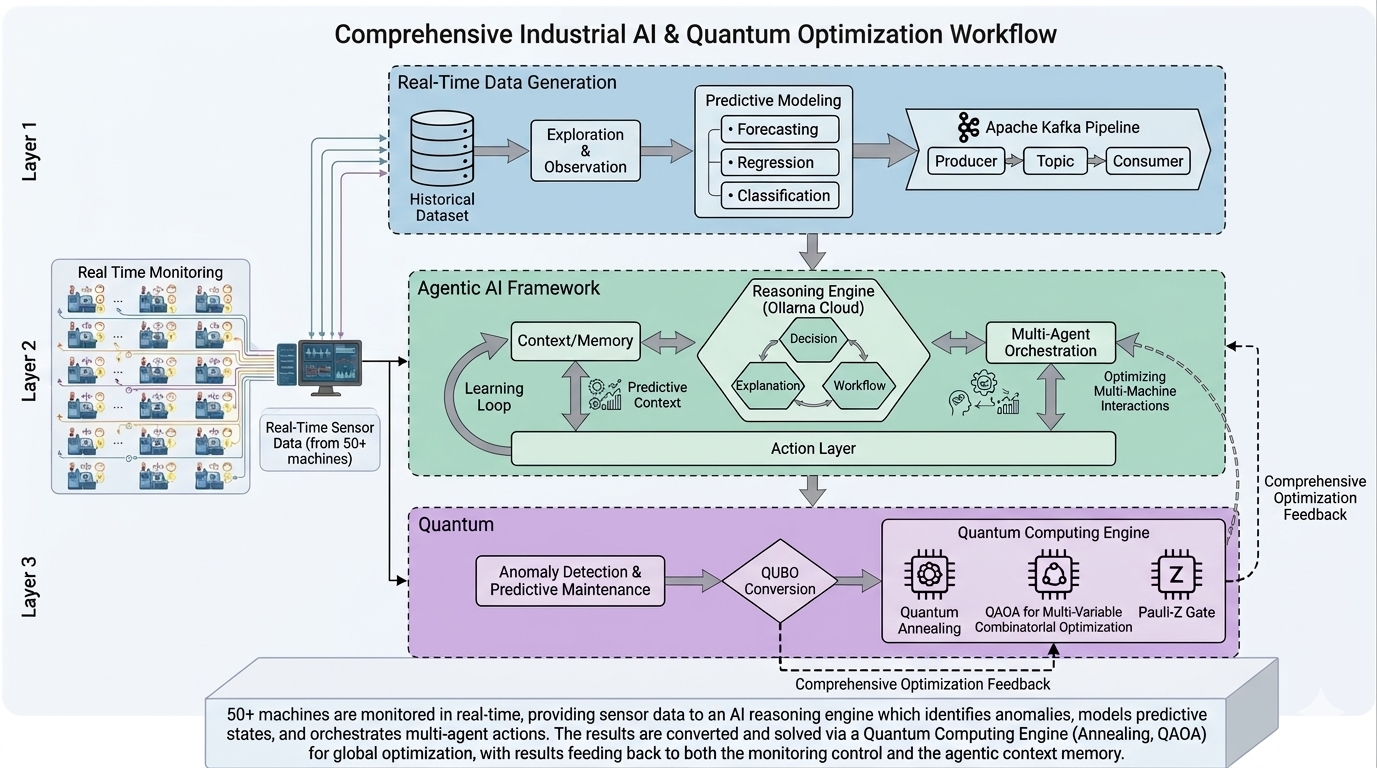
\includegraphics[width=\textwidth]{figures/research_methodology.png}
    \caption{QASAMAP Research Methodology: The three-layer architecture spanning data generation and predictive modelling (Layer~1), Agentic AI Framework with multi-agent LLM orchestration (Layer~2), and Quantum Computing Engine with Annealing, QAOA, and Pauli-Z components (Layer~3).}
    \label{fig:research_methodology}
\end{figure}

\textbf{Layer 1 — Data and Predictive Modelling.} The first layer handles real-time sensor data ingestion via an Apache Kafka pipeline simulation and executes three families of predictive models. A Temporal Graph Convolutional Network (T-GCN) performs spatiotemporal sensor stream forecasting, exploiting a cross-correlation lag graph constructed from the temporal relationships among the 50 monitored machines. The cross-correlation graph comprises 50 nodes and 538 directed edges, with Machine 40 identified as the anchor node based on its highest out-degree centrality. Supervised tree-based ensemble models (XGBoost, LightGBM, CatBoost, HistGradientBoosting) and the TabNet deep tabular model are evaluated for five classification targets (machine status, anomaly flag, failure type, downtime risk, maintenance required) and one regression target (predicted RUL). The empirical motivation for graph-based modelling is grounded in the dataset: temperature (Pearson $r = 0.447$ with anomaly flag) is the most informative single sensor, and the cross-correlation structure reveals predictive relationships between machines that enable machine-wide anomaly propagation.

\textbf{Layer 2 --- Agentic AI Framework.} The second layer implements a multi-agent orchestration system in which specialised LLM-powered agents collaborate to transform sensor evidence and quantum context into operational maintenance decisions. The agentic layer is empirically evaluated through four pre-registered experiments (E1 capability coverage, E3 in-context adaptation, E5 robustness under controlled perturbations, E6 multi-agent vs single-call ablation), with two further experiments (E2 cross-domain cold-start, E4 operator decision quality) documented as deferred future work. Detailed architecture, value-proposition framework, and experimental results are presented in Chapter~5.

\textbf{Layer 3 --- Quantum Computing Engine.} The third layer augments the pipeline with two quantum computing components evaluated on Qiskit Aer statevector simulators with NISQ-honest framing. A Pauli-Z entangled compound encoder maps each machine's five normalised sensor values to a 5-qubit register via $R_Y$ rotations and a CNOT entanglement chain, producing a composite expectation value as the anomaly score (E-Q3). A QAOA-based maintenance scheduler formulates the time-slot assignment problem as a Quadratic Unconstrained Binary Optimisation (QUBO) and is benchmarked against a tuned classical Simulated Annealing baseline and brute-force enumeration (E-Q1). Both experiments test for parity-with-classical at simulator scale; no quantum-advantage claim is made on the QASAMAP problem itself. Detailed encoding, statistical results, and NISQ caveats are presented in Chapter~6.

\subsection{Research Objectives}

This thesis pursues five primary research objectives that collectively address the identified gaps. The first objective is to develop and evaluate a T-GCN-based spatiotemporal forecasting architecture for multi-machine sensor stream prediction, incorporating cross-correlation lag graph construction, machine-wide anomaly propagation, and real-time streaming inference with partial sensor data imputation via the \texttt{AnchorBufferManager}. The second objective is to evaluate and compare classical tree-based ensemble models and TabNet for simultaneous multi-target classification and RUL regression using the 50-machine dataset. The third objective is to implement and demonstrate Pauli-Z multi-sensor encoding, QUBO-based quantum annealing, and QAOA scheduling for maintenance prioritization and slot assignment within an industrial predictive maintenance context. The fourth objective is to design and implement a multi-agent agentic AI system that autonomously orchestrates the complete predictive maintenance decision cycle from sensor event ingestion through maintenance action dispatch, integrating quantum override signals into agent reasoning. The fifth objective is to empirically evaluate the full QASAMAP framework through a three-way comparative study against a traditional rule-based system and an agentic AI system without quantum enhancement, quantifying the independent contributions of the agentic and quantum layers to detection accuracy, response time, machine coverage, downtime reduction, and cost savings.

\subsection{Research Contributions}

The primary contributions of this thesis are as follows. First, a novel spatiotemporal forecasting architecture combining T-GCN with cross-correlation lag graphs is demonstrated to outperform both standalone LSTM (avg.\ R$^2$ = 0.6853) and Hybrid LSTM-GCN (avg.\ R$^2$ = 0.7134) baselines, achieving avg.\ R$^2$ = 0.7702 on a 100,000-reading industrial dataset. Second, a comprehensive benchmark of five supervised learning algorithms across six machine health prediction targets is provided, establishing performance baselines for anomaly detection (best F1 = 0.999), failure type classification (best F1 = 0.880), maintenance prediction (best F1 = 0.872), and RUL regression (best R$^2$ = 0.189). Third, an empirical evaluation of the agentic AI layer against six pre-registered Value Propositions is reported in Chapter~5: Hybrid QASAMAP achieves 55\% capability coverage across eight PdM decision dimensions versus 20\% for Pure ML (Cochran's Q significant on 6 of 8 dimensions, $p < 0.05$), with honest mixed-evidence reporting of in-context adaptation (E3), robustness (E5), and a counter-result on multi-agent specialisation versus single-call (E6) reconciled by a breadth-versus-quality distinction. Fourth, NISQ-honest quantum experiments on Qiskit statevector simulators are reported in Chapter~6: a 5-qubit Pauli-Z entangled compound detector achieves $F1 = 0.290$ at natural anomaly prevalence on QASAMAP test data (best of five baselines, $+0.078$ F1 over its mathematically isolated separable equivalent, McNemar $p < 0.0001$ Bonferroni-corrected), and a simulated QAOA scheduler reaches solution-quality parity with classical Simulated Annealing at depth $p \ge 2$ (Wilcoxon $p = 0.317$ for $p=2$, $p = 0.180$ for $p=3$, $N = 20$ paired instances). No claim of quantum advantage on QASAMAP is made; the quantum positioning is architectural-readiness for the NISQ-Advanced phase (2025--2028), anchored by industrial precedents from Ford Otosan (6$\times$ scheduling speedup) and BASF (7200$\times$ liquid-filling speedup) on adjacent industrial scheduling problems.

\subsection{Thesis Structure}

The remainder of this thesis is organized as follows. Chapter~2 provides a review of the relevant literature across sensor-based anomaly detection, deep learning for predictive maintenance, quantum machine learning, and agentic AI systems. Chapter~3 presents the proposed QASAMAP methodology, including the T-GCN architecture and the high-level multi-layer system design. Chapter~4 reports the dataset description, T-GCN forecasting results, and supervised classification and regression benchmarks. Chapter~5 covers the agentic AI layer with its six Value-Proposition framework and pre-registered experimental evaluation (E1, E3, E5, E6 executed; E2 and E4 deferred). Chapter~6 covers the quantum computing layer with NISQ-honest framing and pre-registered experiments E-Q3 (Pauli-Z entangled compound detection) and E-Q1 (SA versus simulated QAOA scheduling). Chapter~7 provides discussion and analysis of the findings. Chapter~8 concludes with a synthesis of contributions and directions for future research.